\documentclass[11pt, a4paper]{article}

% --- 基本頁面設定 ---
\usepackage[a4paper, top=2.5cm, bottom=2.5cm, left=2cm, right=2cm]{geometry}

% --- 圖片與浮動控制套件 ---
\usepackage{graphicx} 
\usepackage{float} % 修正：加入此套件以支援 [H] 指令

% --- XeLaTeX 專用中文套件 ---
\usepackage{xeCJK}

% 設定中文字體：微軟正黑體 (Windows 內建)
\setCJKmainfont{Microsoft JhengHei}

% 設定英文字體：Arial (Windows 內建)
\setmainfont{Arial}

% --- 數學與表格套件 ---
\usepackage{amsmath}
\usepackage{booktabs}
\usepackage{enumitem}
\setlist[itemize]{label=-}
\usepackage{multicol}

% --- 1. Title (標題) ---
\title{\textbf{Numerical Simulation of Discrete-Time Nonlinear Population Dynamics using Logistic Map in Java}}

% --- 個人資訊 ---
\author{蔡晟旭 \\ 
Student ID: 1113405013 \\
國立澎湖科技大學 資訊工程學系 \\
National Penghu University of Science and Technology}
\date{\today}

\begin{document}

\maketitle

% --- 2. Abstract (摘要) ---
\begin{abstract}
本報告旨在探討非線性動力系統中的邏輯斯諦映射（Logistic Map）在 Java 程式環境下的數值模擬實作。透過物件導向程式設計（OOP）與迭代運算，本研究分析了增長率參數 $r$ 對系統行為的影響，並觀察到從穩定狀態演變至混沌狀態的過程。本實驗同時整合了 GitHub 版本控制與 AI 輔助開發流程，以符合現代軟體工程之學術規範。
\\ \\
% --- 3. GitHub 網址 ---
\textbf{GitHub Repository:} https://github.com/tch107146/JAVA-0303-Assignments-1
\end{abstract}

% --- 4. Keywords (關鍵字) ---
\noindent \textbf{Keywords:} Java Programming, Nonlinear Dynamics, Logistic Map, Iterative Computation, GitHub, Chaos Theory.

\begin{multicols}{2}

% --- 5. Introduction (引言) ---
\section{Introduction}
在計算科學領域中，Java 語言憑藉其類別封裝特性與平台無關性，成為模擬複雜動力系統的理想選擇。本次實驗（Assignment 1）的核心目標在於建立專業的開發環境，並透過實作經典的非線性模型來掌握 Java 的基本語法與迭代邏輯。

% --- 6. Methodology (研究方法) ---
\section{Methodology}
本實驗採用邏輯斯諦映射公式來模擬受限環境下的人口增長行為：
\begin{equation}
x_{n+1} = r \cdot x_n \cdot (1 - x_n)
\end{equation}
其中參數定義如下：
\begin{itemize}
    \item $x_n \in [0, 1]$：第 $n$ 代的人口密度比例。
    \item $r \in [0, 4]$：增長率參數。當 $r$ 增加時，系統會經歷倍週期分叉，最終進入混沌狀態。
\end{itemize}

% --- 7. Implementation Details (實作細節) ---
\section{Implementation Details}
本程式採用 Java 11 進行開發，實作細節如下：
\begin{itemize}
    \item \textbf{Encapsulation}: 建立 \texttt{PopulationModel} 類別。
    \item \textbf{Iterative Logic}: 使用 \texttt{for} 迴圈執行核心運算。
    \item \textbf{I/O Interaction}: 利用 \texttt{java.util.Scanner} 獲取使用者參數。
\end{itemize}

% --- 8. Experimental Results (實驗結果) ---
\section{Experimental Results}
經測試，系統在不同參數下呈現顯著差異：
\begin{enumerate}
    \item 當 $r=2.5$ 時，人口比例迅速收斂至固定穩定值。
    \item 當 $r=3.9$ 時，系統呈現不規則震盪，展現混沌特徵。
\end{enumerate}

% --- 圖片插入部分 ---
\begin{figure}[H] % 現在已經支援 [H] 強制定位
  \centering
  % 檢查圖片是否存在，如果不存在則顯示方框，避免編譯報錯
  \IfFileExists{screenshot.png}{
    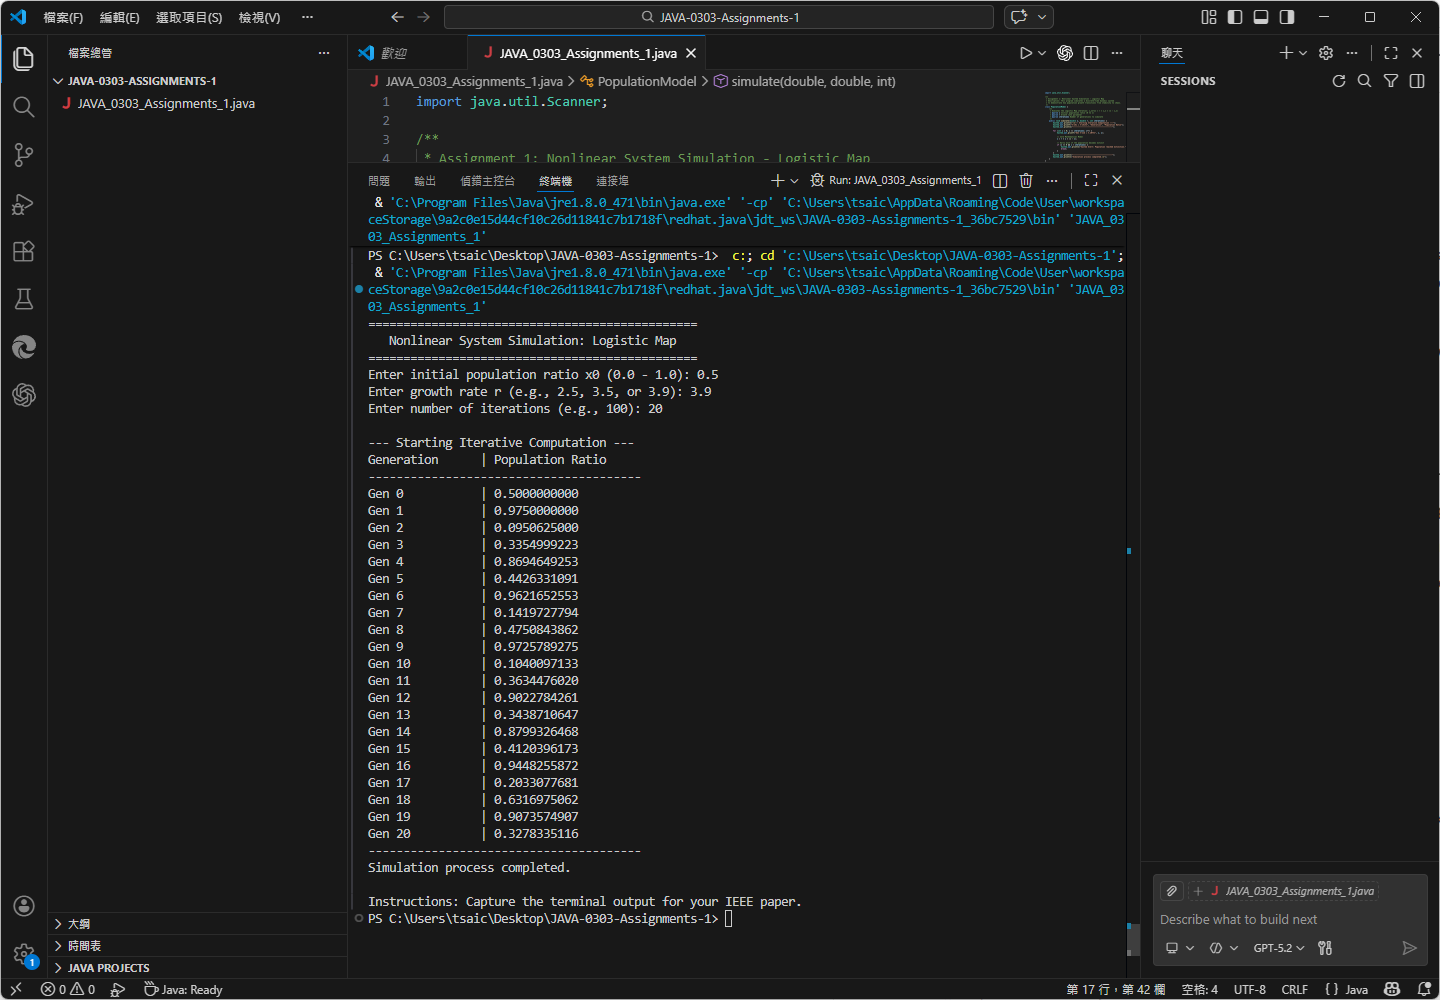
\includegraphics[width=0.9\columnwidth]{screenshot.png}
  }{
    \framebox{\parbox{0.8\columnwidth}{\centering \vspace{1.5cm} [圖片檔案 screenshot.png 缺失] \\ 請將圖片放在本 .tex 檔所在目錄 \vspace{1.5cm}}}
  }
  \caption{Simulation output for $r=3.9$.}
  \label{fig:result}
\end{figure}

% --- 9. Discussion (討論) ---
\section{Discussion}
在實驗過程中觀察到，若初始值 $x_0 = 1.0$，由於公式項 $(1-x_n)$ 歸零，人口比例會立即降至 0。這反映了非線性系統對於初始邊界條件的高敏感度。

% --- 10. Conclusion (結論) ---
\section{Conclusion}
本作業成功完成了從環境建置到學術寫作的完整流程。這不僅強化了 Java 程式實作能力，也學會了如何撰寫正式的工程論文報告。

% --- 11. References (參考文獻) ---
\section{References}
\noindent [1] H. Rui, \textit{Lecture 0: Preliminary Introduction}, NPU, 2025. \par
\noindent [2] Robert M. May, "Simple mathematical models with very complicated dynamics," \textit{Nature}, vol. 261, pp. 459-467, 1976.

\end{multicols}

\end{document}